\section{Tracing Rays} 
I implemented the functions\\
\texttt{bool ClosestIntersection(glm::vec3 start, glm::vec3 dir, const std::vector<Triangle>\& triangles, Intersection\& closestIntersection);}\\
and\\
\texttt{bool RayTriangleIntersection(glm::vec3 start, glm::vec3 dir, const std::vector<Triangle>\& triangles, Intersection\& intersection);}\\ 
as described in the assignment
instructions. To render the image in the \texttt{Draw()} function I then calculate the ray direction for each pixel as \texttt{d=(x-W/2, y-H/2,f)} where I chose 
\texttt{f=500} and as a starting position I chose \texttt{(0,0,-3)}. I set \texttt{W=500} and \texttt{H=500}. 
Then I use \texttt{ClosestIntersection} to calculate the intersections and determine the color of the pixel.
The horizontal/vertical field of view can be calculated as 
\begin{equation}
    \alpha=2*\arctan(\frac{X}{2f})
\end{equation}
where X=H or X=W respectively. With my chosen values this results in a vertical and horizontal field of view of 53\degree.
\begin{figure}[ht]
    \centering
    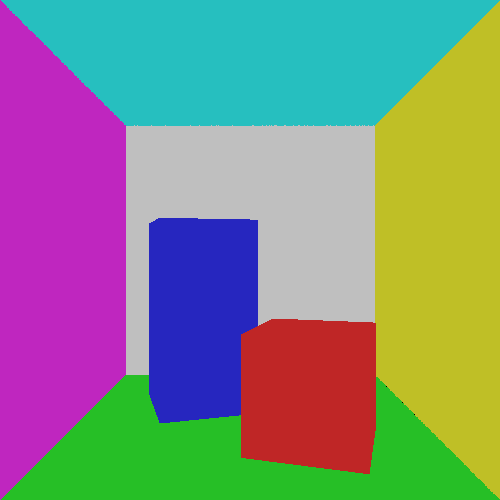
\includegraphics[width=10cm]{screenshots/tracing_rays.png}
\end{figure}
\clearpage

\section{Moving the camera}
To implement camera movement I store a rotation matrix R and the rotation angle. In the update function I then check for key presses:
\begin{itemize}
    \item UP = move camera forwards by decrementing the z value of the camera position
    \item DOWN = move camera backwards by incrementing the z value of the camera position
    \item LEFT = rotate camera to the left by decrementing the yaw
    \item RIGHT = rotate camera to the right by incrementing the yaw
\end{itemize}
I then calculate the rotation matrix with the yaw. In the ray-triangle intersection code I rotate all vertices by multiplication with the R matrix
to get the effect of camera rotation. The camera translation is realized by using the new, translated camera position as ray origin.
\begin{figure}[ht]
    \centering
    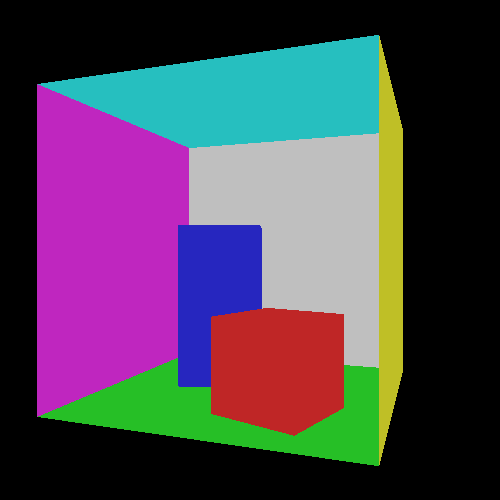
\includegraphics[width=10cm]{screenshots/camera_movement.png}
\end{figure}
\clearpage

\section{Direct Light}
I implemented the function \texttt{glm::vec3 DirectLight(const Intersection\& i)} by using the equations given in the instructions. Then I use 
this function in the Draw function to calculate the color of each pixel.
\begin{figure}[ht]
    \centering
    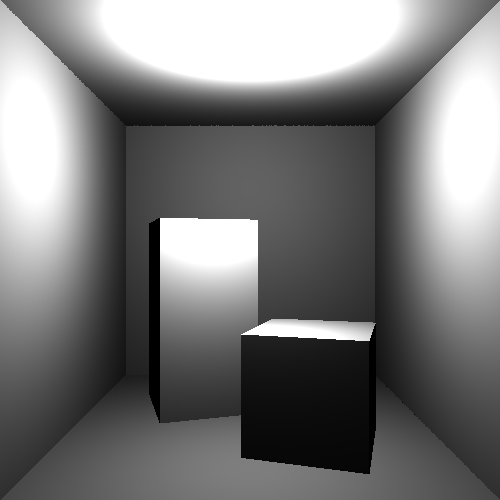
\includegraphics[width=10cm]{screenshots/incoming_light.png}
\end{figure}
\clearpage
\subsection{Moving the light}
To move the light source I implement the following
\begin{itemize}
    \item W = move light forwards by incrementing the z value of the light position
    \item S = move light backwards by decrementing the z value of the light position
    \item D = move light to the right by incrementing the x value of the light position
    \item A = move light to the left by decrementing the x value of the light position
    \item Q = move light down by decrementing the y value of the light position
    \item E = move light up by incrementing the y value of the light position
\end{itemize}
\begin{figure}[ht]
    \centering
    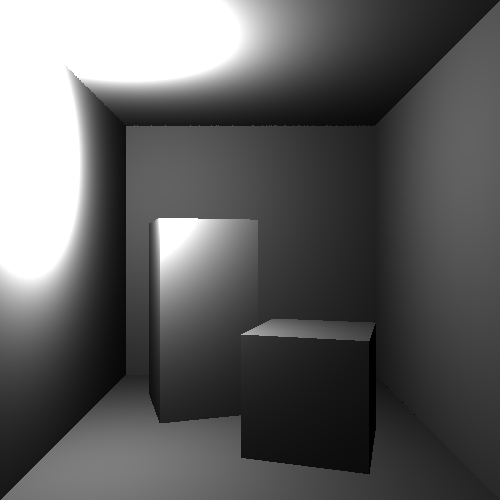
\includegraphics[width=10cm]{screenshots/move_light.png}
\end{figure}
\clearpage
\subsection{Direct illumination without shadows}
I updated the calculation of the color in the Draw function with the given equation to obtain direct illumination without shadows
\begin{figure}[ht]
    \centering
    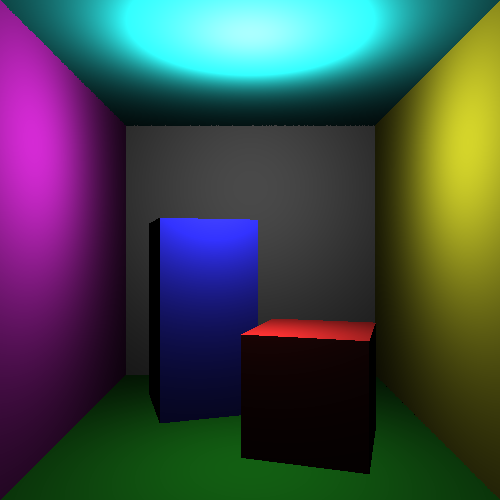
\includegraphics[width=10cm]{screenshots/direct_without_shadows.png}
\end{figure}
\clearpage
\subsection{Direct illumination with shadows}
I updated the DirectLight function to cast a ray from the intersection point to the light source. If there is an intersection with another object 
before that ray reaches the light source, the object to render is in the shadow. While implementing this I had the problem of artifacts because the
the calculations resulted in an immediate self intersection. I solved this by ignoring the current object for intersection test of shadow ray. 
An even better solution would be to move the origin of the shadow ray a tiny bit away from the surface.
\begin{figure}[ht]
    \centering
    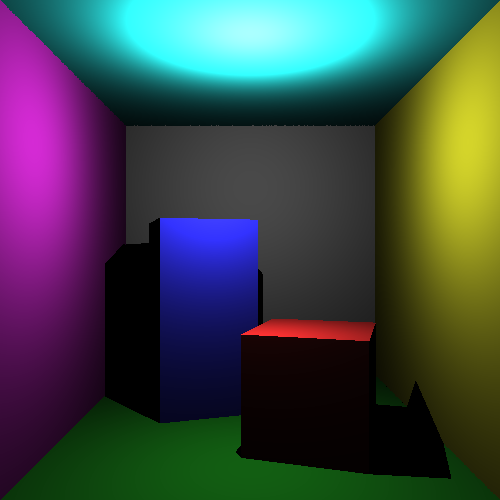
\includegraphics[width=10cm]{screenshots/direct_with_shadows.png}
\end{figure}
\clearpage
\subsection{Indirect illumination}
I implemented the indirect light as described in the instructions. The picture below shows my final result.
\begin{figure}[ht]
    \centering
    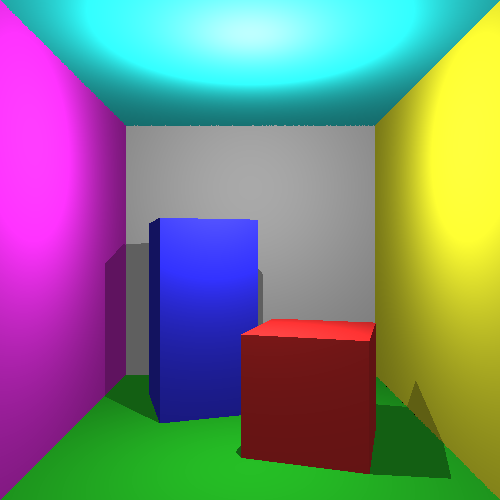
\includegraphics[width=10cm]{screenshots/indirect_illumination.png}
\end{figure}
